\documentclass[11pt]{article}
\usepackage{graphicx}
\usepackage{hyperref}
\usepackage{amsmath}
\usepackage{amsthm}
\usepackage{amssymb}
%\usepackage[all=normal,floats,leading,paragraphs,charwidths,tracking,wordspacing]{savetrees}
\usepackage{float}
%\usepackage[version = 4]{mhchem}
\usepackage{multirow}
\usepackage{commath}
\usepackage{booktabs}
\usepackage{subcaption}
\usepackage{natbib}
%\renewcommand{\arraystretch}{1.2}
\usepackage{setspace}
\onehalfspacing
\usepackage[nottoc,numbib]{tocbibind}
\usepackage{siunitx}
\sisetup{detect-all}
\DeclareSIUnit{\atm}{atm}
\usepackage{listings}
\usepackage{color} %red, green, blue, yellow, cyan, magenta, black, white
\definecolor{mygreen}{RGB}{28,172,0} % color values Red, Green, Blue
\definecolor{mylilas}{RGB}{170,55,241}
\usepackage[a4paper,margin=20mm]{geometry}
\numberwithin{equation}{section}
\setlength{\parskip}{\baselineskip}
\setlength{\parindent}{0pt}
\hypersetup{
    colorlinks=true,
    linkcolor=black,
    filecolor=black,      
    urlcolor=black,
    citecolor=black
}
\urlstyle{same}
\lstset{language=Matlab,%
    %basicstyle=\color{red},
    breaklines=true,%
    morekeywords={matlab2tikz},
    keywordstyle=\color{blue},%
    morekeywords=[2]{1}, keywordstyle=[2]{\color{black}},
    identifierstyle=\color{black},%
    stringstyle=\color{mylilas},
    commentstyle=\color{mygreen},%
    showstringspaces=false,%without this there will be a symbol in the places where there is a space
    numbers=left,%
    numberstyle={\tiny \color{black}},% size of the numbers
    numbersep=9pt, % this defines how far the numbers are from the text
    emph=[1]{for,end,break},emphstyle=[1]\color{red}, %some words to emphasise
    %emph=[2]{word1,word2}, emphstyle=[2]{style},    
}
\begin{document}
\begin{titlepage}
    \begin{center}
        \vspace*{1cm}
             
        MECH0020 Individual Project\\
        2021/22
 
        \vspace{1.5cm}

        {\LARGE \textbf{Designing a Lap Simulator for the Shell Eco-marathon} \par}
             
        \vspace{1.5cm}
 
        Student: Hasha Humayon Dar
        
        \vspace{0.25cm}

        Supervisor: Professor Tim Baker
        
        \vfill

        Word count: 3565

        \vspace{0.25cm}

        University College London\\
        Torrington Place\\
        LONDON WC1E 7JE
             
    \end{center}
 \end{titlepage}
\newpage
\section*{Declaration}
I, Hasha Humayon Dar, confirm that the work presented in this report is my own. Where information has been derived from other sources, I confirm that this has been indicated in the report.
\section*{Abstract}
The development of simulating performance parameters for racing vehicles has become increasingly important in a digital world. Simulations provide highly customisable virtual environments to test components, changes and strategies. Hence, the development of software that can give an accurate idea of a vehicle's performance in a variety of configurations would prove to be an advantage. Traditionally, the UCL Racing Team has conducted in-person testing of their vehicles at race tracks or similar. However, due to COVID-19, this has become difficult in the past two years. Virtual testing can provide a cheaper, more time efficient means of testing. The development of a virtual model of the vehicle would allow the team to test various changes to the vehicle, without having to prototype and arrange for in-person testing. 

This report focuses on building a performance based model of the UCL Racing Shell Eco-marathon vehicle, which generates a lap time for the vehicle. The Shell Eco-marathon is a competition at the school and university level for students focusing on energy optimisation in vehicles. The aim of the competition is to develop new innovations in energy efficiency for vehicles on the road with the idea of reducing carbon emissions \citep{shell1}.
\section*{Acknowledgements}
Throughout this project I have received a great deal of support and assistance. First and foremost, I would like to thank my supervisor, Prof. Tim Baker, whose expertise was invaluable in the development of this project. 

I would also like to acknowledge the support of the UCL Mechanical Engineering Department, which champions innovation through projects like these. Their facilities and teaching have proven to be an incredible asset for this project. 

I would also like to thank my parents for their continuous and unwavering support of my studies and activities. Thank you for always being there for me. Finally, there are my friends, who were a source of support and distraction, both of which proved very useful for deliberating over problems and to rest my mind from academia. Thank you to you all.
\newpage
\tableofcontents
\listoffigures
\listoftables
\newpage
\section{Project background and problem}
UCL Racing currently competes in the Shell Eco-marathon in the `prototype' category. Hence, this simulator will focus on reproducing the performance characteristics of a vehicle in this class. The vehicles is a small hydrogen-powered single-seater, designed with a focus on attaining ultra-efficiency through the optimisation of the aerodynamic and performance characteristics of the vehicle.

For an ultra-energy-efficient vehicle, there are many sources of inefficiency. Some of them are aerodynamic drag (air resistance), friction drag (from the road surface) and losses in the powertrain (electricity generation, mechanical losses) \citep{Wei2019}. The design itself of the car must be optimised to increase its performance such as the weight of the vehicle \citep{Tsirogiannis2019}.

A problem that arises when investigating and modelling these variables is that there is no way of testing certain performance characteristics within the holistic context of the competition virtually. Currently, to test newly designed components and its overall impact on the performance of the vehicle, the part must be prototyped and installed on the vehicle, and then experimentally tested. This presents a problem as this is costly, time-consuming and constrains the number of prototypes that can be made.

A transient, dynamic lap simulator will allow the analysis of the vehicle's various performance characteristics. This will allow the team to optimise and prototype designs much more effectively. The team would be able to test the vehicle on the final test track, without the cost of being there physically. This simulator will also allow vehicular strategies to be tested, as virtually any track can be inputted and tested. 

As creating a virtual model of a vehicle can become an extremely complex process depending on the resolution and level of accuracy required. This simulator will focus specifically on the overall performance parameters of the vehicle, considering the car as a homogeneous unit, rather than an assembly of the various components that make up a vehicle. 
\section{Objectives}
The simulator should meet the following objectives:
\begin{itemize}
    \item Process and store track data
    \item Process and store vehicle data
    \item Calculate forces acting upon the vehicle and sources of inefficiency during a transient simulation of the vehicle running around the track.
    \item Output data on various performance parameters
    \item Generate a lap time for the vehicle
\end{itemize}
As this simulator is designed to be used by students in the coming years as tool to inform them on their design choices, an element of ease of use is also important. Good practices such as well written and laid out code is important to ensure that outside users can understand it and make their own adjustments. The software should also be computationally efficient, allowing for use on most machines without requiring large amounts of computer resources. 
\section{Methodology and design}
\subsection{Track data}
It was decided that a simulator which can simulate a vehicle for any track was important to allow for a wider array of testing scenarios. Hence, the simulator is designed to use only x-y-z-coordinate data as an input. This maps the trajectory of the vehicle as it goes around the track. The most efficient route around a racetrack is the `racing line'. Racing line coordinate data can be found for many tracks. For testing purposes, racing line data was used from Alexander Heilmeier's Github repository \citep{heilmeier_2022}. Calculations are then made on various aspects of the track. This includes the radius of curvature of the track, which is calculated using geometrical principles.
\begin{figure}[H]
    \centering
    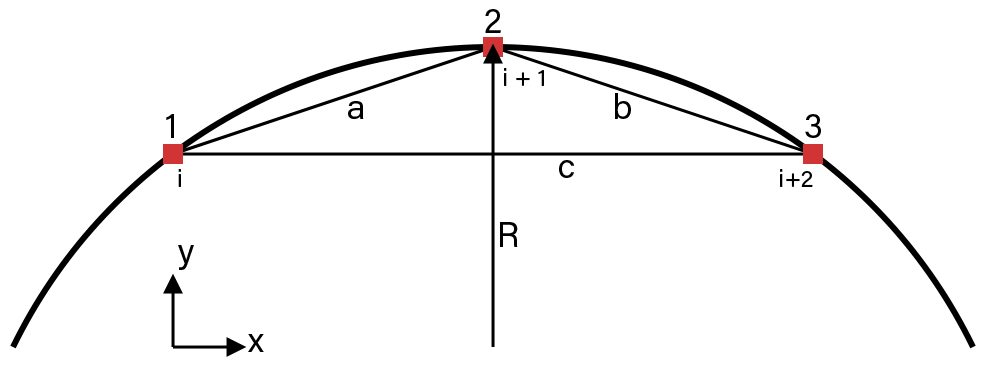
\includegraphics[width = 0.8\textwidth]{./img/radiusOfCurvature.png}
    \caption{Radius of curvature calculation.}
\end{figure}
The code indexes the x-y coordinates of three sequential track points and calculates the radius of curvature by use of the following equations.
\begin{gather}
    a = \sqrt{\left(x_2 - x_1\right)^2 + \left(y_2 - y_1\right)^2}\\
    b = \sqrt{\left(x_3 - x_2\right)^2 + \left(y_3 - y_2\right)^2}\\
    c = \sqrt{\left(x_3 - x_1\right)^2 + \left(y_3 - y_1\right)^2}\\
    q = \dfrac{a^2 + b^2 - c^2}{2ab}\\
    R = \dfrac{c}{2\sqrt{1 - q^2}}
\end{gather}
The slope between adjacent track points is calculated using trigonometry.
\begin{figure}[H]
    \centering
    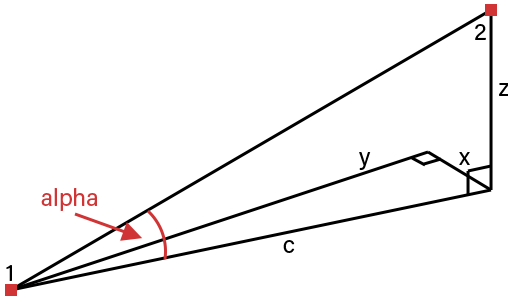
\includegraphics[width = 0.6\textwidth]{./img/trackSlope.png}
    \caption{Track slope calculation.}
\end{figure}
\begin{gather}
    c = \sqrt{\left(x_2 - x_1\right)^2 + \left(y_2 - y_1\right)^2}\\
    z = z_2 - z_1\\
    \alpha = \arctan\left(\dfrac{z}{c}\right)
\end{gather}
After the calculation of the radius of curvature and slope at the discrete steps along the length of the track, these values are concatenated with the cumulative distance of the track. This will allow us to interpolate the values of the above variables during our simulation. 
\subsection{DC motor model}
The car is powered by a small DC motor, attached to the rear wheel. A Simscape DC motor model was used to output torque as function of a virtual throttle position. This allows for a highly customisable power unit and control system.
\begin{figure}[H]
    \centering
    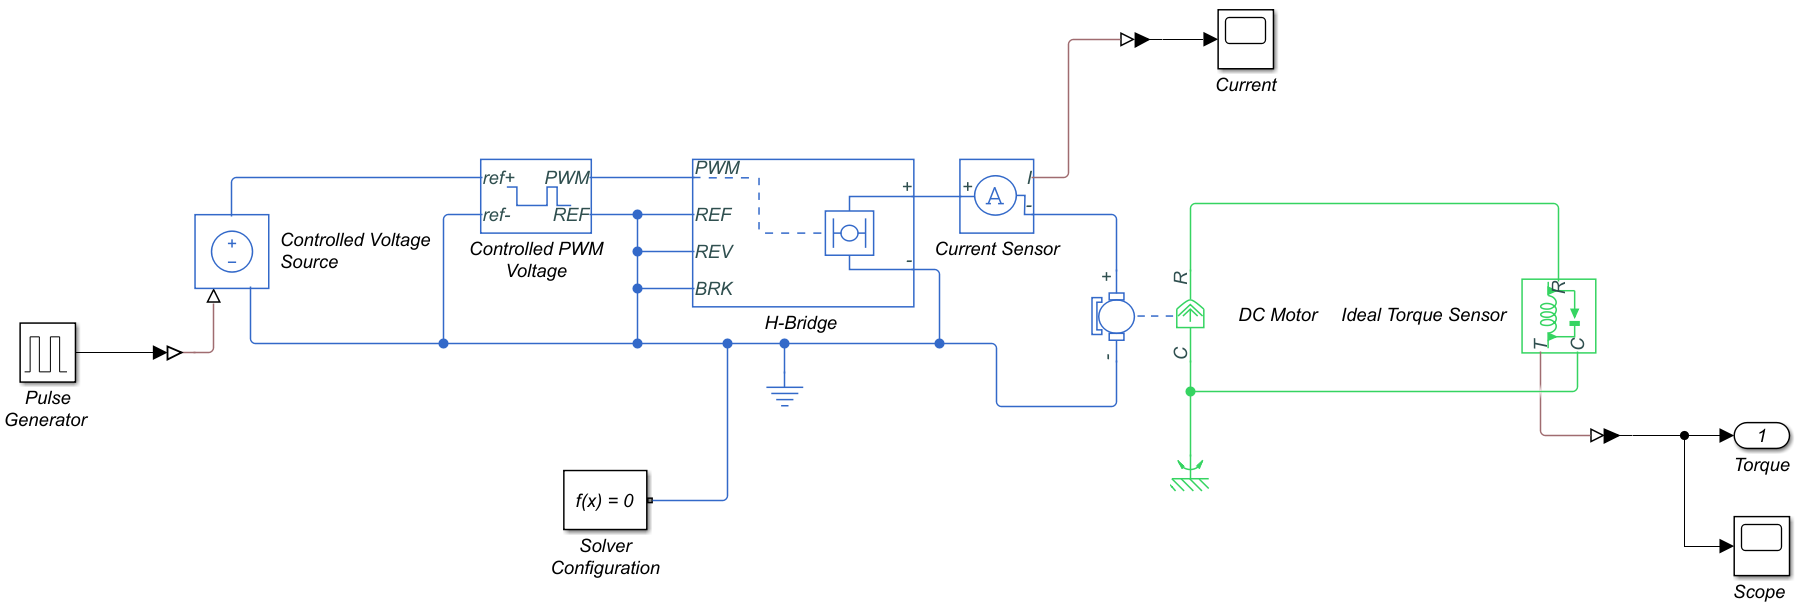
\includegraphics[width =\textwidth]{./img/DCMotorModel.png}
    \caption{DC motor model.}
\end{figure}
The throttle input can be inputted into the simulation via the use of an array as a function of the time. A PWM controller is then used as an input to the motor driver, which provides current to the DC motor. The Simscape DC motor block allows the motor parameters to be defined as a function of the rated load and speed. Electrical characteristics such as the armature inductance, and rated supply voltage are defined here as well. Mechanical characteristics such as the rotor inertia and damping can also be added. A torque sensor is then used to provide our output.
\subsection{Transmission model}
The vehicle utilises a simple transmission with only one drive ratio. Transmission inefficiencies stemming from mechanical losses can be modelled using a variable gain factor. The drive ratio converts the torque from the DC motor shaft to the torque applied at the wheel.
%\begin{figure}[H]
%   \centering
%    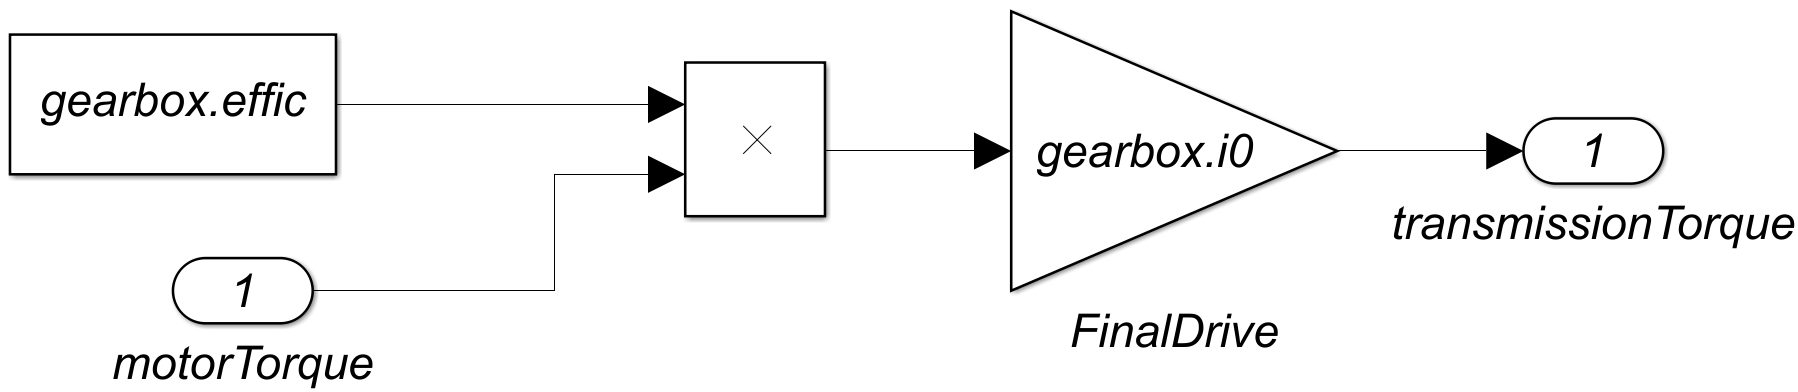
\includegraphics[width =\textwidth]{./img/transmissionModel.png}
%    \caption{Transmission model.}
%\end{figure}
\begin{gather}
    \tau_{t} = \left( \tau_m \cdot \eta_{g} \right) \times \texttt{gearbox.i0}
\end{gather}
where $\tau_m$ is the motor torque, $\eta_{g}$ is the gearbox efficiency and $\tau_t$ is the transmission torque.
\subsection{Vehicle model}
\subsubsection{Force analysis}
\begin{figure}[H]
    \centering
    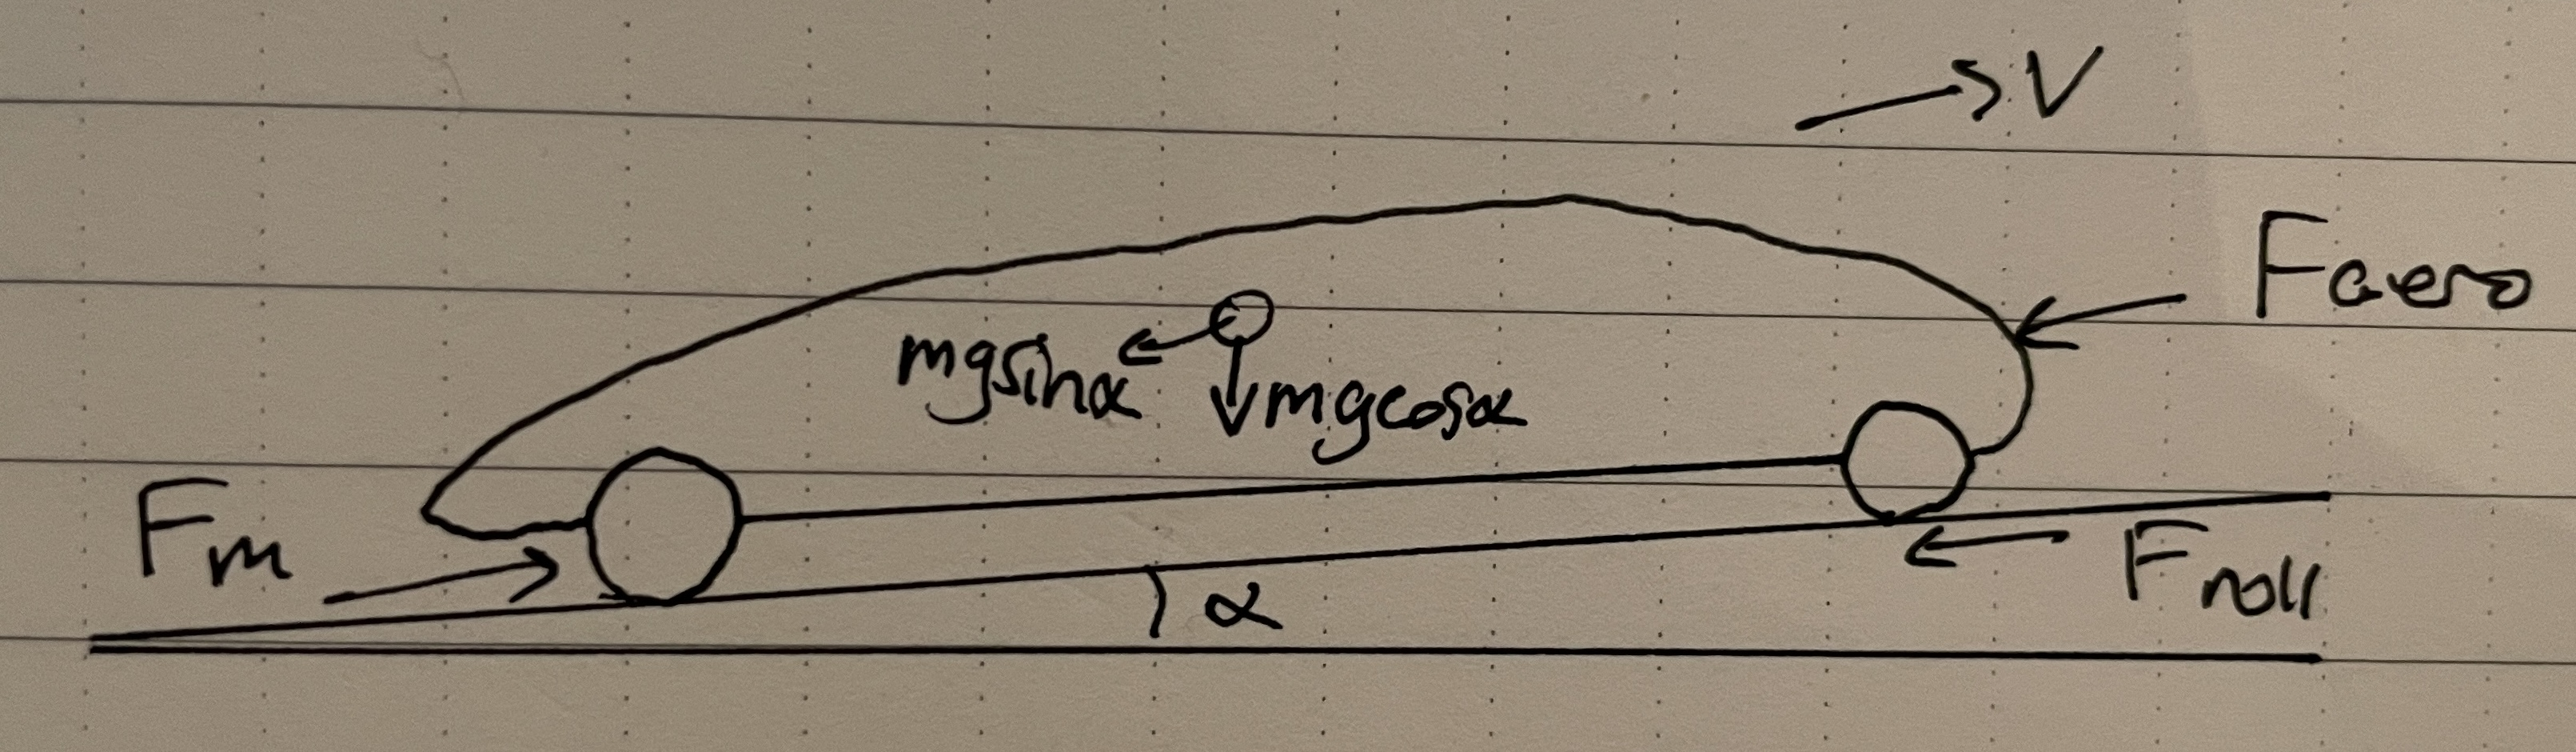
\includegraphics[width = \textwidth]{./img/vehicleSketch1.jpg}
\end{figure}
A force model for conventional internal combustion vehicles have been developed extensively before. Kamalakkannan outlines a model for analysing the straight line performance of a vehicle \citep{balaji}. As these same forces are applicable to our vehicle, an outline of the force analysis is outlined below. 

The vehicle's movement can be described by the longitudinal forces:
\begin{gather}
    F_t = F_i + F_a + F_s + F_r \label{forces1}
\end{gather}
\begin{itemize}
    \item $F_m$ - traction force in \si{\newton}
    \item $F_i$ - inertial force in \si{\newton}
    \item $F_a$ - aerodynamic force in \si{\newton}
    \item $F_s$ - slope force in \si{\newton}
    \item $F_r$ - rolling resistance in \si{\newton}
\end{itemize}
Our transmission torque must then be converted into the force applied to the road $F_m$. This can be found by dividing transmission torque by wheel radius. 
\begin{gather}
    F_m = \dfrac{\tau_t}{\texttt{tyre.rwd}}
\end{gather}
where $\tau_t$ is the torque supplied after gearing and \texttt{tyre.rwd} is the radius of the rear tyre. The force that can be applied to the road from the wheel is limited by the friction coefficient applicable to the contact patch of the tyre. The maximum friction force can be calculated as:
\begin{equation}
    F_f = m_c \cdot g \cdot \mu_a\cdot \texttt{tyre.load} 
\end{equation}
where $m_c$ is the combined vehicle mass, $g$ the gravitational acceleration, $\mu_a$ is the tyre friction coefficient and \texttt{tyre.load} is the rear axle load coefficient. The model compares the $F_t$ and $F_f$, saturating at $F_f$. If a force above $F_f$ is applied, this would result in wheelspin. Due to the slow speeds of the vehicle, wheel slip in this regard is not expected.
Inertial effects must also be considered in our model. These can be modelled as:
\begin{gather}
    F_i = m_c \cdot a_v \label{forces2}
\end{gather}
where $a_v$ is the vehicle acceleration.

The aerodynamic drag force can be calculated as:
\begin{gather}
    F_a = \frac{1}{2} \cdot A \cdot \rho \cdot c_d \cdot v^2
\end{gather}
where $A$ is the vehicle frontal area, $\rho$ is the air density, $c_d$ is the drag coefficient and $v$ is the vehicle velocity.

The force generated by the vehicle's mass on a slope can be calculated as:
\begin{gather}
    F_s = m_c \cdot g \cdot \sin\left(\alpha\right)
\end{gather}
where $\alpha$ is the angle of road slope from true horizontal. 

Rolling resistance can be calculated as:
\begin{gather}
    F_r = m_c \cdot g \cdot c_r \cdot \cos \left(\alpha\right)
\end{gather}
where $c_r$ is the road load coefficient.

Substituting \ref{forces2} into \ref{forces1}:
\begin{gather}
    a_v = \frac{1}{m_c}\left(F_t - F_a - F_s - F_r\right)
\end{gather}
Integrating gives us our velocity:
\begin{gather}
    v = \frac{1}{m_c}\int\left(F_t - F_a - F_s - F_r\right)\dif t
\end{gather}
\begin{figure}[H]
    \centering
    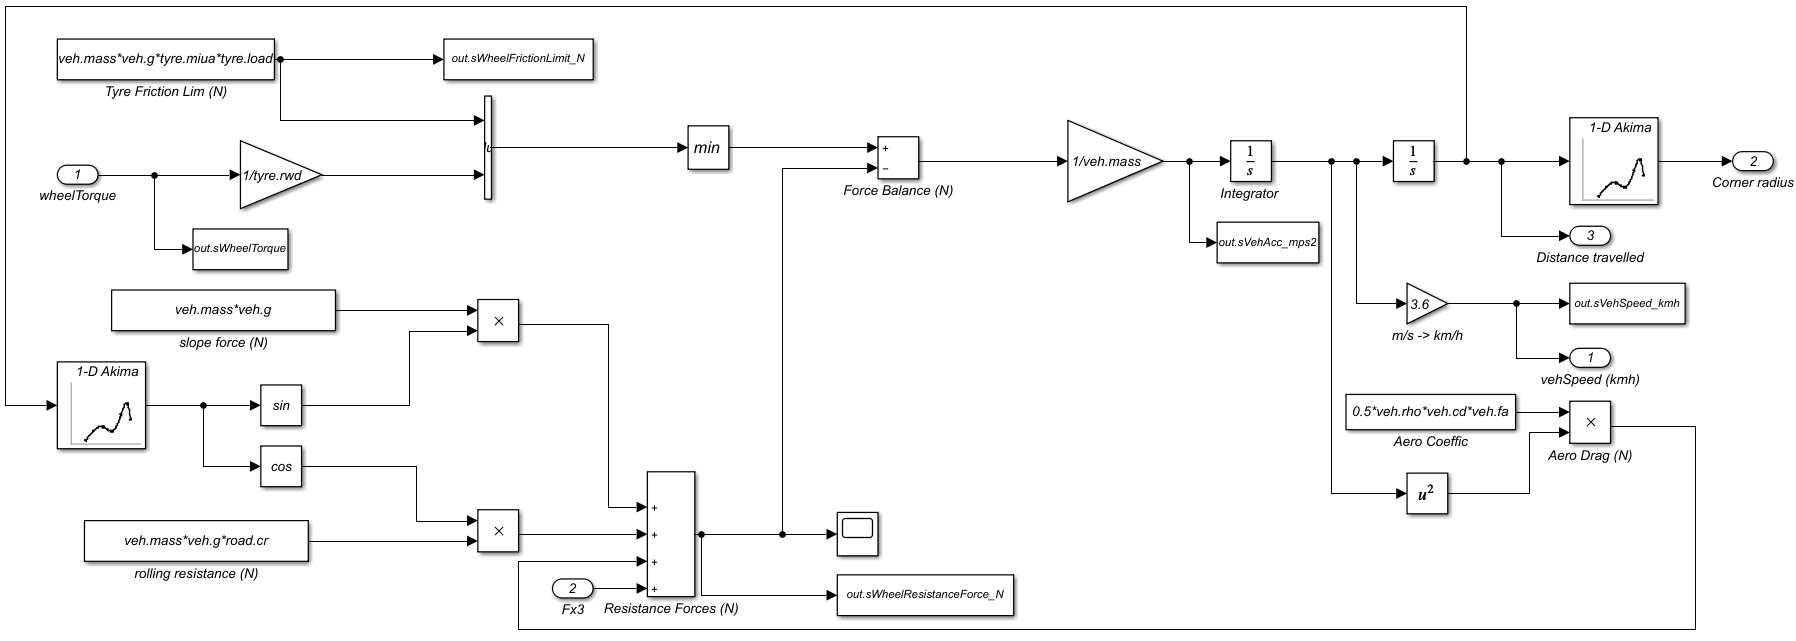
\includegraphics[width = 0.8\textwidth]{./img/vehicleModel.png}
    \caption{Vehicle force modelling in Simulink. Here we can see how a force balance is created and calculated transiently during our test.}
    \label{vehicleBlock}
\end{figure}
\subsubsection{Tyre model}
A tyre model must be implemented to assess the effects of cornering on the vehicles velocity. We start with the vehicle geometry itself. An implementation for a truck vehicle is outlined in \citep{BECKERS2020102360}. This model outlines the use of the Pacejka Magic Formula for calculating tyre forces as a function of slip.
\begin{figure}[H]
    \centering
    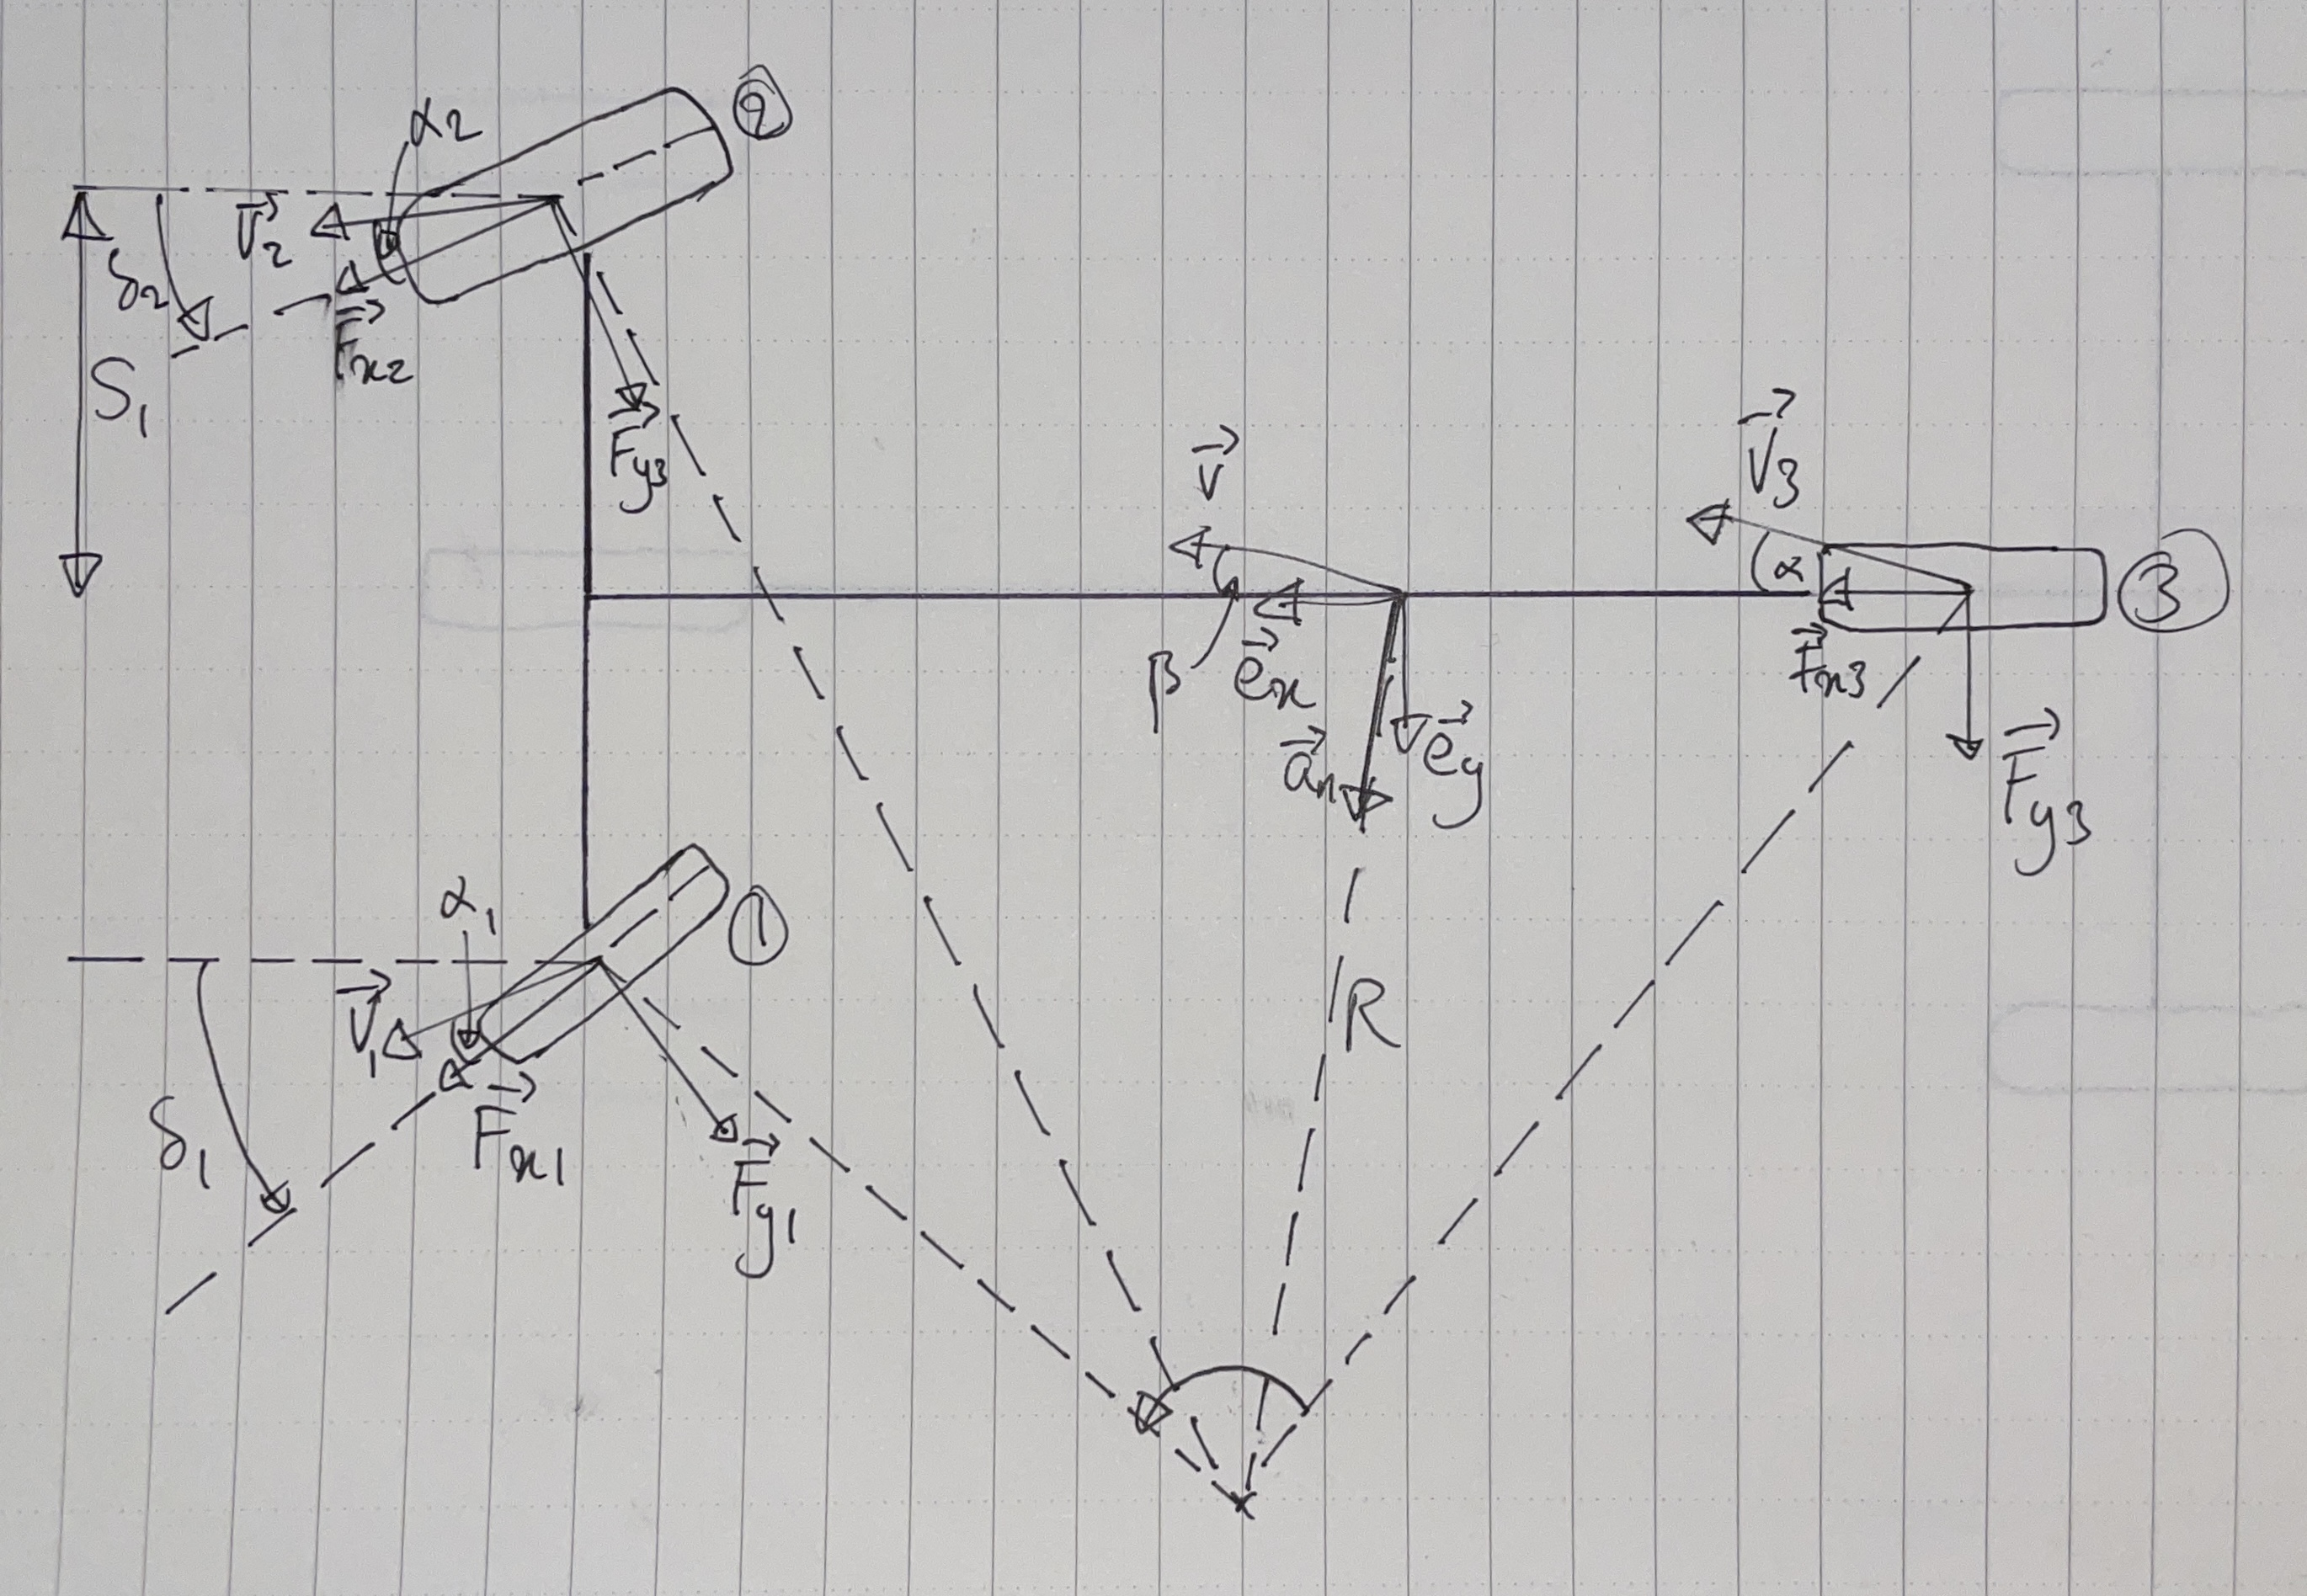
\includegraphics[width = \textwidth]{./img/vehicleSketch2.JPG}
    \caption{Vehicle diagram during cornering. We can see that a fixed vehicle-axis system is defined from the centre of mass ($\vec{e}_{x/y}$). Velocity vectors for the centre of mass and three tyres are also shown ($\vec{V}_i$). Force vectors acting upon the tyres are shown ($\vec{F}_{yi}$). The radius of the turn and the cornering angles of the tyres are shown ($R, \, \delta_i$). We can also see the angles that the velocity vectors make with their respective fixed axes ($\alpha, \, \beta$).}
\end{figure}
We first start with the velocity components of the centre of mass:
\begin{gather}
    v_x = V\cos\beta\\
    v_y = -V\sin\beta\\
    \omega_z = \frac{V}{R}
\end{gather}
where $v_x$ is the longitudinal centre of mass velocity, $v_y$ is the lateral centre of mass velocity and $\omega_z$ is the yaw rate of the vehicle. The velocity vector of the vehicle can be stored in the following matrix.
\begin{gather}
    \vec{v} = \underline{v}\cdot \vec{\underline{e}} = \begin{bmatrix}
        v_x & v_y & 0
    \end{bmatrix} \begin{bmatrix}
        \vec{e}_x\\
        \vec{e}_y\\
        \vec{e}_z
    \end{bmatrix}
\end{gather}
where $\vec{\underline{e}}$ represents unit vectors describing the vehicle's fixed axis system in relation to the centre of mass. Similarly, we can also define the position of the tyres.
\begin{gather}
    \vec{p}_i = \underline{p}_i \cdot \vec{\underline{e}} \textrm{ for } i = 1,\, 2, \, 3
\end{gather}
where $\vec{p}_i$ is a column vector with the position coordinates of a given tyre. These are a function of the front and rear wheelbases ($l_f$ and $l_r$) and the half of the front axle length ($s_1$).

We can then multiply our velocity matrix with a transformation matrix to attain the local tyre velocities:
\begin{gather}
    \underline{v}_i = \begin{bmatrix}
        \cos\delta_i & \sin\delta_i & 0\\
        -\sin\delta_i & \cos\delta_i & 0\\
        0 & 0 & 1
    \end{bmatrix} \begin{pmatrix}
        \vec{v} + \begin{bmatrix}
            0\\
            0\\
            \omega_z
        \end{bmatrix} \times \underline{p}_i
    \end{pmatrix} \textrm{ for } i = 1, \, 2, \, 3
\end{gather}
This rotation matrix can be defined as follows:
\begin{gather}
    \vec{A}(\delta_i) = \begin{bmatrix}
        \cos\delta_i & \sin\delta_i & 0\\
        -\sin\delta_i & \cos\delta_i & 0\\
        0 & 0 & 1
    \end{bmatrix}
\end{gather}
and rotates the velocity vector from the vehicle fixed axis to the tyre fixed frame with $\delta_i$ as an input. We can calculate the value of $\delta_i$ via Ackermann's steering relation \citep{Kageyama1}.
\begin{gather}
    \delta_1 = \arctan\left(l \left(\frac{l}{\tan\delta}-s_1\right)^{-1}\right)\\
    \delta_2 = \arctan\left(1 \left(\frac{l}{\tan\delta}+s_1\right)^{-1}\right)
\end{gather}
where $l$ is the total wheelbase of the vehicle. As our rear wheel is fixed, we do not need to rotate the velocity vector. We can now find our tyre side slip angles ($\alpha_i$) and longitudinal slip ratios ($\kappa_i$) by looking at the respective velocity components:
\begin{gather}
    \alpha_i = \arctan\left(\dfrac{-v_{y,i}}{\abs{v_{x,i}}}\right) \textrm{ for } i = 1, \, 2, \, 3\\
    \kappa_i = -\dfrac{v_{x,i}-r_{e,i}\omega_i}{\abs{v_{x,i}}} \textrm{ for } i = 1, \, 2, \, 3
\end{gather}
where $r_{e,i}$ is the effective tyre radius as a function of the vertical force acting on the tyre ($F_{z,i}$). We can also neglect longitudinal slip of the front tyres as they are not driven. 

Let us now consider the load transfers laterally and longitudinally. The acceleration of the centre of mass can be written as:
\begin{gather}
    a_x = \sin\beta \cdot \frac{V^2}{R}\\
    a_y = \cos\beta \cdot \frac{V^2}{R}
\end{gather}
The pitch moment and roll moment of the vehicle can be defined as:
\begin{gather}
    M_{pitch} = -a_x \cdot h \cdot m_c\\
    M_{roll} = a_y \cdot h \cdot m_c
\end{gather}
where $h$ is the height of the centre of mass from the ground. When load transfer occurs from rear to front, we can represent the change in vertical force via:
\begin{gather}
    \Delta F_{z,pitch} = \frac{M_{pitch}}{l_f + l_r}
\end{gather}
At the front of the vehicle, we can calculate the change in vertical force from lateral load transfer via:
\begin{gather}
    \Delta F_{z,front} = k_{dist} \frac{M_{roll}}{2s_1}
\end{gather}
We can now calculate the vertical forces applicable to the tyres:
\begin{gather}
    F_{z,1} = \frac{l_r}{2l}mg - \Delta F_{z,front} + \frac{1}{2} \Delta F_{z,pitch}\\
    F_{z,2} = \frac{l_r}{2l}mg + \Delta F_{z,front} + \frac{1}{2} \Delta F_{z,pitch}\\
    F_{z,3} = \frac{l_f}{l}mg - \Delta F_{z,pitch}\\
\end{gather}
To model the forces applicable to the tyres when cornering, we can use a Pacejka's Magic Formula \citep{pacejka2012tire}. This is a simplified tyre model, which characterises the non-linear response of a tyre during cornering. The function outputs the lateral and longitudinal force vectors $F_{x,i}$ and $F_{y,i}$ as a function of the slip conditions ($\alpha_i$ and $\kappa_i$), which are important in realising sources of energy loss in our vehicle system.
\begin{table}[H]
    \centering
    \begin{tabular}{@{}lll@{}}
        \toprule
        Variable & Value & Description\\
        \midrule
        \texttt{p.tyre1.R0} & \SI{0.5}{\meter} & Free tyre radius\\
        \texttt{p.tyre1.Fz0} & \SI{4000}{\newton} & Tyre nominal force\\
        \texttt{p.tyre1.kz} & \SI{109000}{\newton\per\meter} & Tyre vertical stiffness\\
        \texttt{p.tyre1.pCx1} & \SI{1.6}{} & Shape factor \texttt{Cfx} for long. forces\\
        \texttt{p.tyre1.pDx1} & \SI{0.75}{} & Long. friction \texttt{mux} at $F_{z,nom}$\\
        \texttt{p.tyre1.pDx2} & \SI{-0.05}{} & Variation of friction \texttt{mux} with load\\
        \texttt{p.tyre1.pKx1} & \SI{15}{} & Long. slip stiffness $\frac{\texttt{KFx}}{F_z}$\\
        \texttt{p.tyre1.pCy1} & \SI{1.3}{} & Shape factor \texttt{Cfy} for lateral forces\\
        \texttt{p.tyre1.pDy1} & \SI{0.7}{} & Lateral friction coefficient at $F_{z,0}$\\
        \texttt{p.tyre1.pDy2} & \SI{-0.1}{} & Lateral friction coefficient dependency on $F_z$\\
        \texttt{p.tyre1.pEy1} & \SI{0.15126}{} & Lateral curvature \texttt{EFy} at $F_{z,nom}$\\
        \texttt{p.tyre1.pEy2} & \SI{0}{} & Lateral curvature dependency on $F_z$\\
        \texttt{p.tyre1.pKy1} & \SI{7.702}{} & Peak cornering stiffness $\texttt{Cfa} = \texttt{pKy1}\cdot F_{z0}$\\
        \texttt{p.tyre1.pKy2} & \SI{2.13}{} & Vertical force at which peak \texttt{Cfa} occurs\\
        \bottomrule
    \end{tabular}
    \caption{Table to show tyre parameters for Magic Formula.}
\end{table}
\begin{figure}[H]
    \centering
    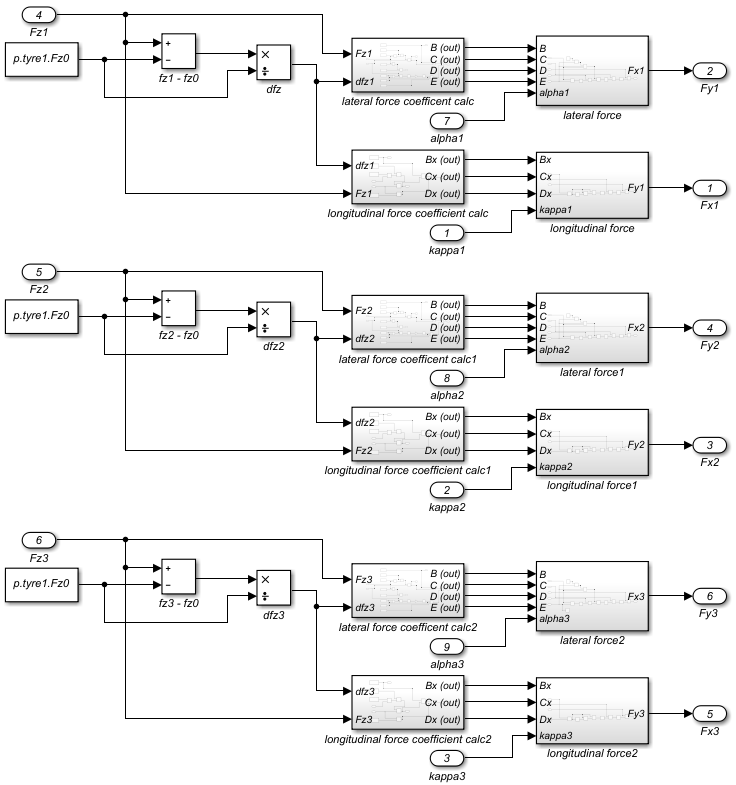
\includegraphics[width = 0.6\textwidth]{./img/magicTyreCalcs.png}
    \caption{Simulink block diagram of Magic Formula. Here we see our inputs of $F_{z,i}$, $\alpha_i$ and $\kappa_i$. Our outputs are $F_{x,i}$ and $F_{y,i}$.}
\end{figure}
Our constants can be calculated as follows:
\begin{gather}
    \texttt{dfz} = \frac{F_z - F_{z,0}}{F_{z,0}}\\
    Cy = \texttt{pCy1}\\
    Cx = \texttt{pCx1}\\
    \texttt{muy} = \texttt{pDy1} + \texttt{pDy2} \cdot \texttt{dfz}\\
    \texttt{mux} = \texttt{pDx1} + \texttt{pDx2} \cdot \texttt{dfz}\\
    Dy = F_z \cdot \texttt{muy}\\
    Dx = F_z \cdot \texttt{mux}\\
    Ey = \texttt{pEy1} + \texttt{pEy2}\cdot \texttt{dfz}\\
    Kx = \texttt{pKx1}\cdot F_z\\
    \texttt{Cfa} = \texttt{kPy1}\cdot F_{z,0} \cdot \sin\left(2\arctan\left(\frac{F_z}{F_{z,0}\cdot \texttt{pKy2}}\right)\right)\\
    By = \frac{\texttt{Cfa}}{Cy \cdot Dy}\\
    Bx = \frac{Kx}{Cx \cdot Dx}
\end{gather}
The forces can be calculated as:
\begin{gather}
    F_y = Dy\cdot \sin\left(Cy \cdot \arctan\left(\left(1 - Ey\right)\cdot By \cdot \alpha + Ey \cdot \arctan\left(By\cdot \alpha\right)\right)\right)\\
    F_x = Dx \cdot \sin\left(Cx \arctan\left(Bx \cdot \kappa -\left(Bx \cdot \kappa - \arctan\left(Bx \cdot \kappa\right)\right)\right)\right)
\end{gather}
$F_x$ is outputted to our vehicle force balance block and used in the calculation for our vehicle speed. This can be seen in Figure \ref{vehicleBlock}.
%\begin{figure}[H]
%    \centering
%    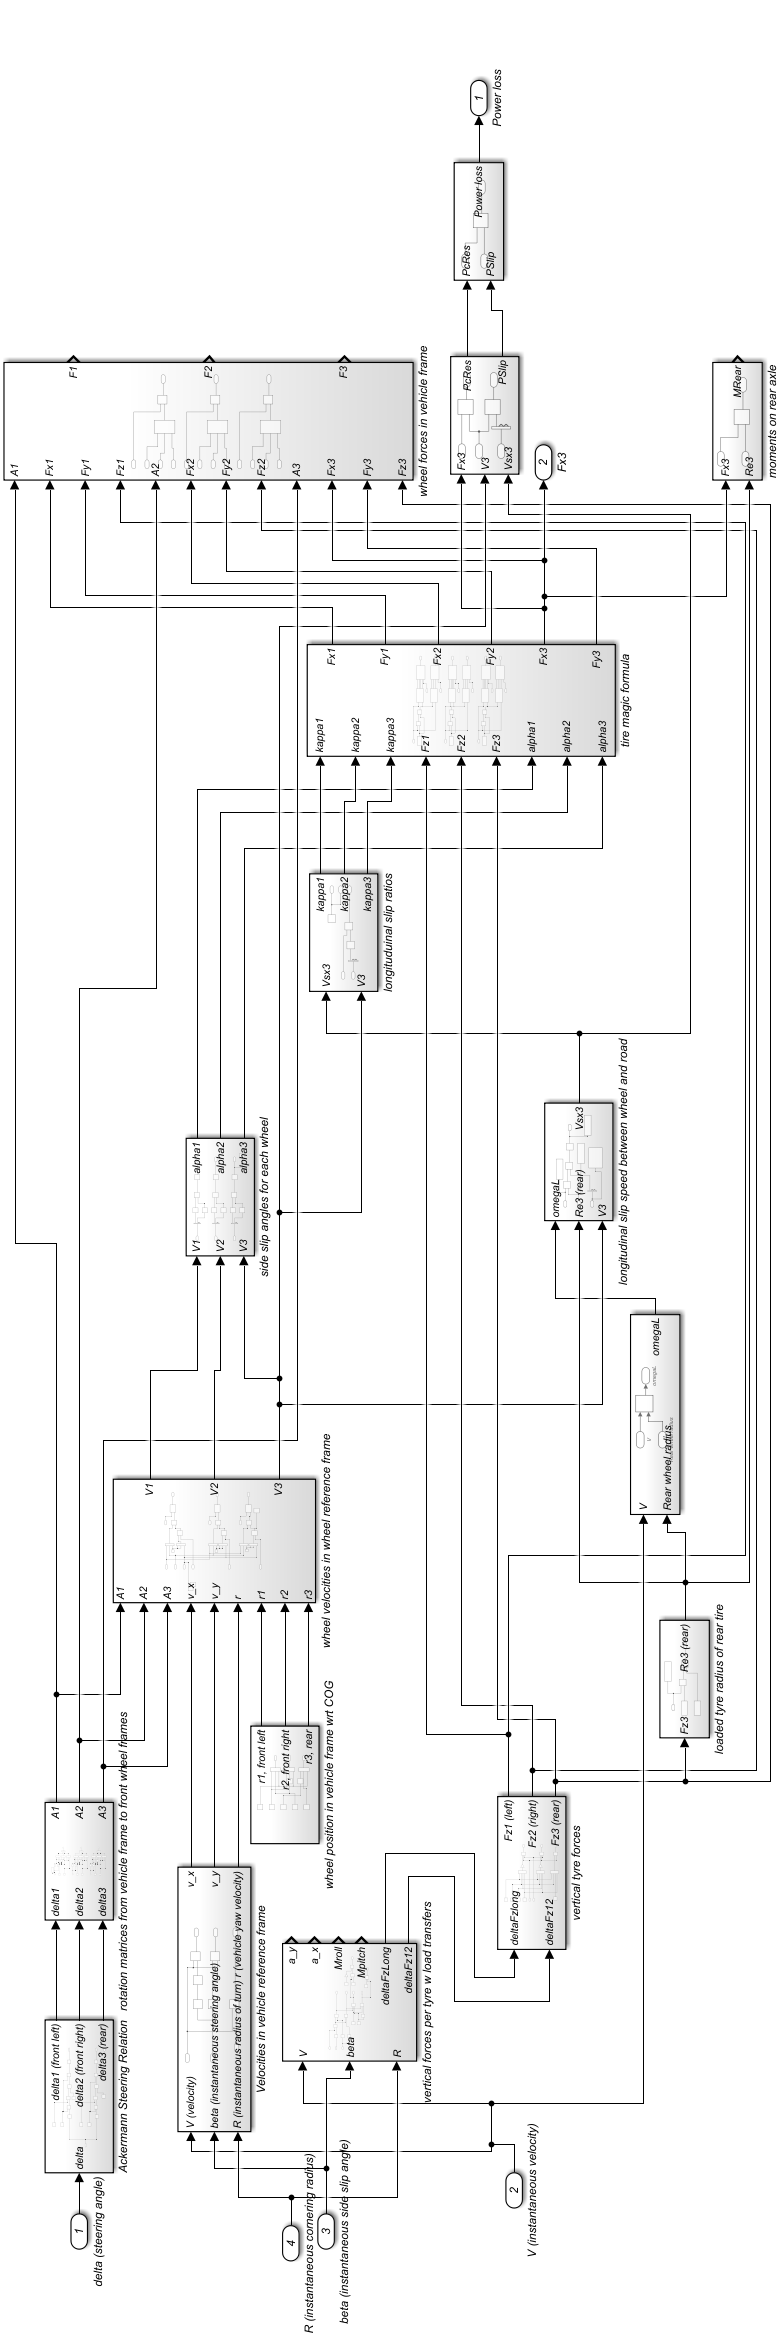
\includegraphics[height = 0.9\textheight]{./img/tyreModel.png}
%    \caption{Block model diagram of tyre model. The inputs are calculated via interpolation from our track data by also utilising the current distance travelled as an index value. }
%\end{figure}
\section{Results}
The simulation is run in Simulink and a \texttt{stop} block is utilised once a lap is completed (indexed via distance travelled and compared to the calculated track length). The chosen track used in this simulation was the Brands Hatch Circuit in the UK.  
\begin{table}[H]
    \centering
    \begin{tabular}{@{}lll@{}}
        \toprule
        Parameter & Value & Symbol \\
        \midrule
        Combined vehicle mass & \SI{165}{\kilo\gram} & $m_c$\\
        Wheelbase & \SI{2}{\meter} & $l$\\
        Centre of mass position from front & \SI{1}{\meter} & $l_f$\\
        Centre of mass height above ground & \SI{0.3}{\meter} & $h$\\
        Distance between tyre and centre line of vehicle & \SI{0.3}{\meter} & $s_1$\\
        \bottomrule
    \end{tabular}
    \caption{Parameters used for simulation.}
\end{table}
\begin{figure}[H]
    \centering
    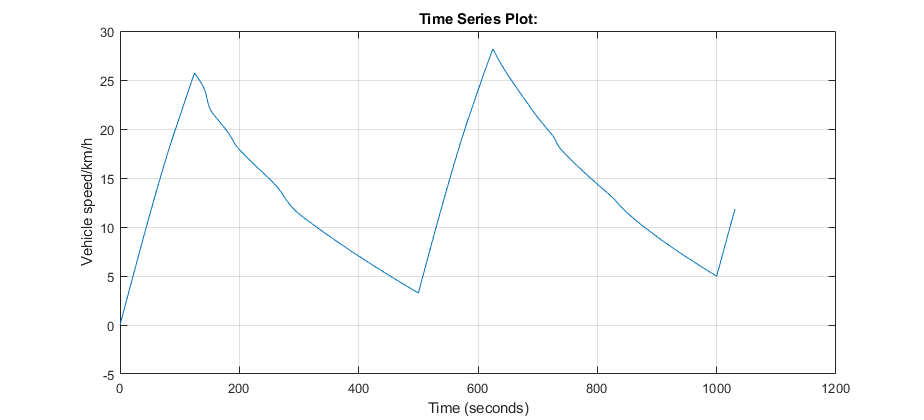
\includegraphics[width = 0.8\textwidth]{./img/vehSpeed.png}
    \caption{Graph to show vehicle speed over course of the track.}
    \label{vehSpeed}   
\end{figure}
In Figure \ref{vehSpeed}, we can see that the strategy employed is three short bursts of acceleration at the start, middle and end of the track. We can see the effect that cornering has on the vehicle's velocity especially in the non-driven phases of the vehicle's lap. As the corner radius increases, we see a steeper drop in vehicle velocity. As the car reduces in speed, we see that the vehicle acceleration decreases, which is a result of resistive forces decreasing in magnitude. The lap time generated for this simulation was \SI{1030}{\second} - approximately 17 minutes. The track length is \SI{3878}{\meter}, therefore our average velocity for the lap is \SI{13.7}{\kilo\meter\per\hour}.
%\begin{figure}[H]
%    \centering
%    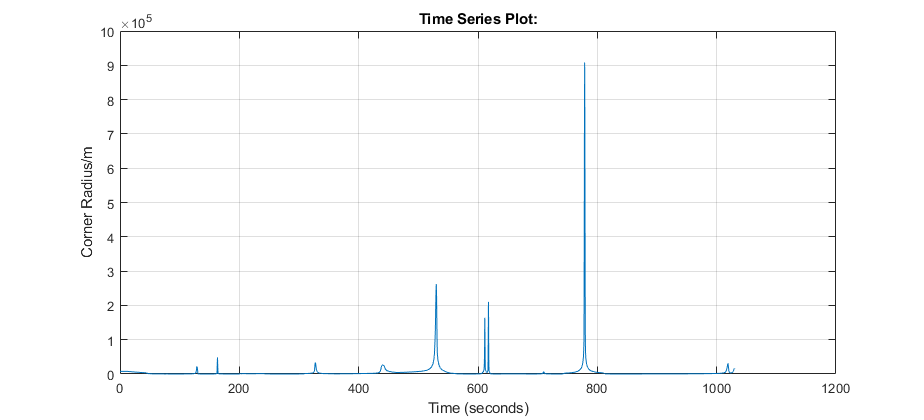
\includegraphics[width = 0.8\textwidth]{./img/trackRadius.png}
%    \caption{Graph to show analysis of track curvature. Peaks highlight regions of the track which are straight.}    
%\end{figure}
\begin{figure}[H]
    \centering
    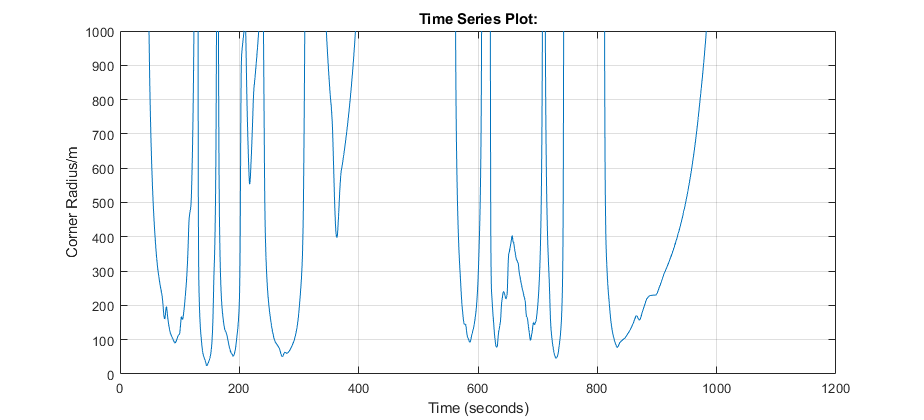
\includegraphics[width = 0.8\textwidth]{./img/trackRadius2.png}
    \caption{Graph to show analysis of track curvature. Troughs highlight regions of the track which are highly curved. Depending on the magnitude of the track radius and the overall shape of the trough, we can infer the overall type of corner (e.g. hairpin or gentle curve).}
    \label{trackCurve}
\end{figure}
In Figure \ref{trackCurve}, we can see the instantaneous track curvature at the position of the vehicle during the simulation. This aligns with our speed plot, as regions with high track curvature decelerate the vehicle. 
\begin{figure}[H]
    \centering
    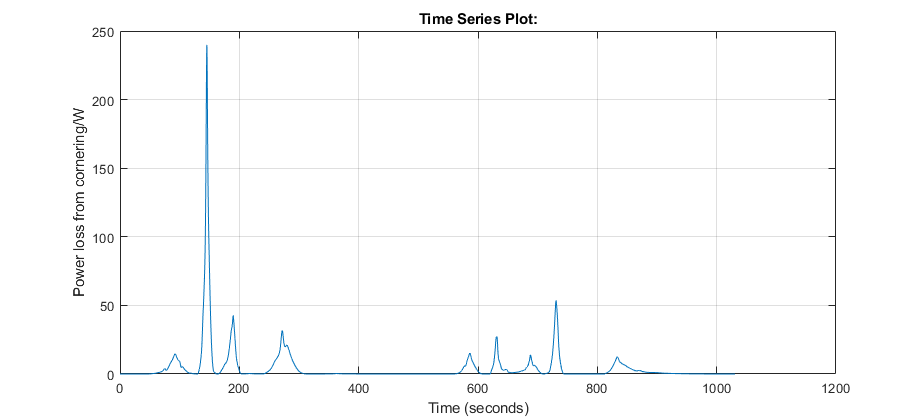
\includegraphics[width = 0.8\textwidth]{./img/powerLossCornering.png}
    \caption{Graph to show analysis of power loss due to cornering. }
    \label{powerLoss}
\end{figure}
in Figure \ref{powerLoss}, we can see the power loss due to cornering. The highest peak here represents the hairpin at turn two of Brands Hatch, which poses a significant loss in energy for the vehicle. We can also see that subsequent turns on the track result in less energy loss. This can be attributed to the slower speed at which some of them are attacked. 
\section{Discussion}
\subsection{Track model}
The track data is processed well by the application. Due to the use of interpolation and matrices, we can store large amounts of track data and process it for any given time step. A further step to add here would be atmospheric conditions of the track. Some of these are already modelled, such as the air density. However, temperature and wind are not considered in this model. Due to the slow speeds of the vehicle, a strong wind may have non-negligible effects on the vehicle's velocity. Hence, the model would need to be improved to consider these effects. Temperature change within the tyres also effects its properties. We know via empirical testing that there is a change in temperature of the tyres during the course of the lap. The effects of these temperature changes could be modelled to improve the accuracy of the model. One factor not considered in the track data is the bank angle of turns. This would have an effect on the vehicle's cornering acceleration and would either improve/deteriorate lap time.

\subsection{Drivetrain model}
The model provides a good starting framework for simulating the Shell Eco car's vehicle performance. The DC motor model provides the basis for the powertrain of our vehicle. Its flexibility allows us to input any strategy for a given track. This can be developed into an algorithmic function, which can optimise a race strategy for a particular track. However, some limitations include that accurate motor data must be obtained for it to map the real-life performance. This can be performed with physical tests using a dynamometer. Another limitation is the model does not account for the source of energy. A fuel cell is responsible for providing energy to the motor and on-board systems. Additional features can also be implemented into the model if need be such as regenerative braking and its subsequent effect on energy efficiency. Subsequent development of this model would allow for this to be modelled and an accurate figure for the energy efficiency of the vehicle can be obtained. Similarly, the transmission model would require further testing to ascertain the true efficiency. This can be done in two ways: either by modelling sources of inefficiency or via empirical testing. As the model is simple, empirical testing may be a good way of keeping the computational complexity of the model low.  

\subsection{Force model}
The force balance incorporates the major forces at play during the lap of the vehicle. However, some improvements may include the inclusion of aerodynamic lift and downforce. These would change the effective normal force on the vehicle. Due to the design choices of the Shell Eco car, drag reduction is the primary principle, hence drag inducing aerodynamic components such as spoilers and splitters are not employed on the car. The ability to model these would prove useful to the application to increase its robustness. We can also consider effects such as the small change in frontal area during the cornering phase as the vehicle's centreline is no longer aligned with the velocity vector. Another factor to consider is road conditions. Variable road conditions as a function of the track distance may prove useful in modelling a wet/dry track or a track with differing road surfaces. Further testing would also be required to fine tune certain parameters in the force balance to ensure accuracy of the model. This can be achieved via computational analysis such as computational fluid dynamics (CFD) or empirical testing.

Another area of improvement would be the complexity of the dynamics model. Currently the model only considers the vehicle as a single point of mass. Increasing the fidelity of the model by adding the locations of various of point masses and generating a mass function would aide accuracy. However, this would require additional pre-processing and analysis. Another factor to consider would be vehicle suspension effects. These were not modelled but by increasing the degrees of freedom of the model, these can also be modelled. Another area to consider would be the effect of manual braking. This is not typical in the course of a lap of a Shell Eco-marathon race, hence its effects were not considered. 

\subsection{Tyre model}
The tyre model represents the biggest source of complexity for the model. This has the adverse effect of increasing the runtime of the application. By using lookup tables and pre-processed data, the runtime of the application could be improved. Another source of inaccuracy is the tyre parameters themselves. Pacejka's Magic Formula is an empirical tyre model and requires a variety of tyre parameters to be defined to obtain accurate results. Therefore, without empirical testing of the tyres used on the Shell Eco-car, these parameters may represent a source of inaccuracy. 

\subsection{Conclusion}
As per the objectives of the model, the application can process and store the track data, store and track the vehicle's performance data, run a simulation of the vehicle around a given track and output time-based data on any given variable, and finally the lap-time is also calculated. Further testing will be required to ensure that the model is functioning appropriately. This model can be used by the UCL Racing team to test their car in a virtual environment, to ascertain the performance of a given prototype. Refinements to design choices can then be made. The use of MATLAB and Simulink will allow for easy further development by other persons as these are taught modules in the UCL Mechanical Engineering course. Simulink's user interface is easy to use and the use of commented code and blocks will aide other persons in understanding the functions of specific subsystems and assemblies. The system is still in its first steps and more work will be needed to refine it to a useful simulation tool that can replace physical testing.
\newpage
\bibliographystyle{agsm}
\bibliography{./bib/MECH0020refs.bib}
\end{document}